\section{Comentarios: ¿Qu\'e es esto?}
En la gu\'ia hay detalles sobre instalaci\'on y manejo de comandos, as\'i como descripciones paso a paso y aclaraciones para comprender
las cosas un poco m\'as y no cometer errores al momento de usar PyQt5. Si sufre ansiedad de c\'odigo, probablemente no deber\'ia empezar por aqu\'i, sino por los ejemplos.
\\
Se agradece toda colaboraci\'on o contribuci\'on para con el \href{https://github.com/nicotrozzo/pyqt5-tutorials}{Repositorio de GitHub}, siguiendo el normal flujo de trabajo de Git con Fork y Pull-Request.

\section{Requisitos: ¿Qu\'e necesito para empezar?}

\begin{itemize}
    \item \textbf{Python 3:} Hay que instalar Python... fijate \href{https://www.python.org/}{ac\'a}.
    \item \textbf{PyCharm:} Hay otras opciones como VSCode, Atom, SublimeText, Eclipse, Notepad++, Bloc de notas, del color que quieras... Se recomienda PyCharm, fijate \href{https://www.jetbrains.com/pycharm/}{ac\'a}.
\end{itemize}

\textbf{Nota importante:} seg\'un el proceso de instalaci\'on suele hacerse de forma autom\'atica o no, pero puede ser que necesites usar comandos en la consola de Windows ejecutando scripts de Python que son muy usados,
como pip principalmente, o el propio int\'erprete de Python. Si no te funciona, es porque no lo ten\'es configurado en las variables de entorno del sistema, fijate c\'omo \nameref{error_de_consola}.

\begin{figure}[H]
    \centering
    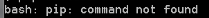
\includegraphics[scale=1]{imagenes/cmd/cmd_error.PNG}
    \caption{Error en la ejecuci\'on desde consola con PIP}
\end{figure}

\section{Instalaci\'on: ¿Qu\'e tengo que instalar?}
\begin{itemize}
    \item \textbf{PyQt5:} Es necesario instalar este paquete. B\'asicamente es una adaptaci\'on del framework QtCreator original empleado en C++ para Python, puede ser que la documentaci\'on en este \'ultimo lenguaje este un poco incompleta.
    Instalamos PyQt5 ejecutando en consola de comandos de Windows, o en la consola de Linux, el comando:
    \begin{center}
        \textbf{pip install PyQt5}
    \end{center}

    \item \textbf{PyQt5-tools/QtDesigner:} Las herramientas de dise\~no QtDesginer, entre otras, para usar con este framework hay que instalarlas con otro comando:
    \begin{center}
        \textbf{pip install pyqt5-tools}
    \end{center}
\end{itemize}

\section{Comandos para consola de windows}

\subsection{¿No te funcionan?}
\label{error_de_consola}
Para que Windows pueda ejecutar un script, bash o alg\'un ejecutable pasando argumentos al programa desde la consola simplemente utilizando una palabra clave, es necesario
que est\'e registrado en las variables de entorno. 
\\
\textbf{Nota importante:} si bien abajo explico c\'omo agregar variables de entorno, es un tema interesante, sirve para otras cosas y tiene v\'inculo con el mecanismo de Python
para importar un paquete o m\'odulo en forma absoluta, podr\'ias \href{https://rootear.com/windows/variable-entorno-windows}{mirarme}, o \href{https://es.ccm.net/contents/652-variables-de-entorno}{a mi}, o tambi\'en \href{https://norfipc.com/inf/variables-entorno.html}{a mi}.


\begin{figure}[H]
    \centering
    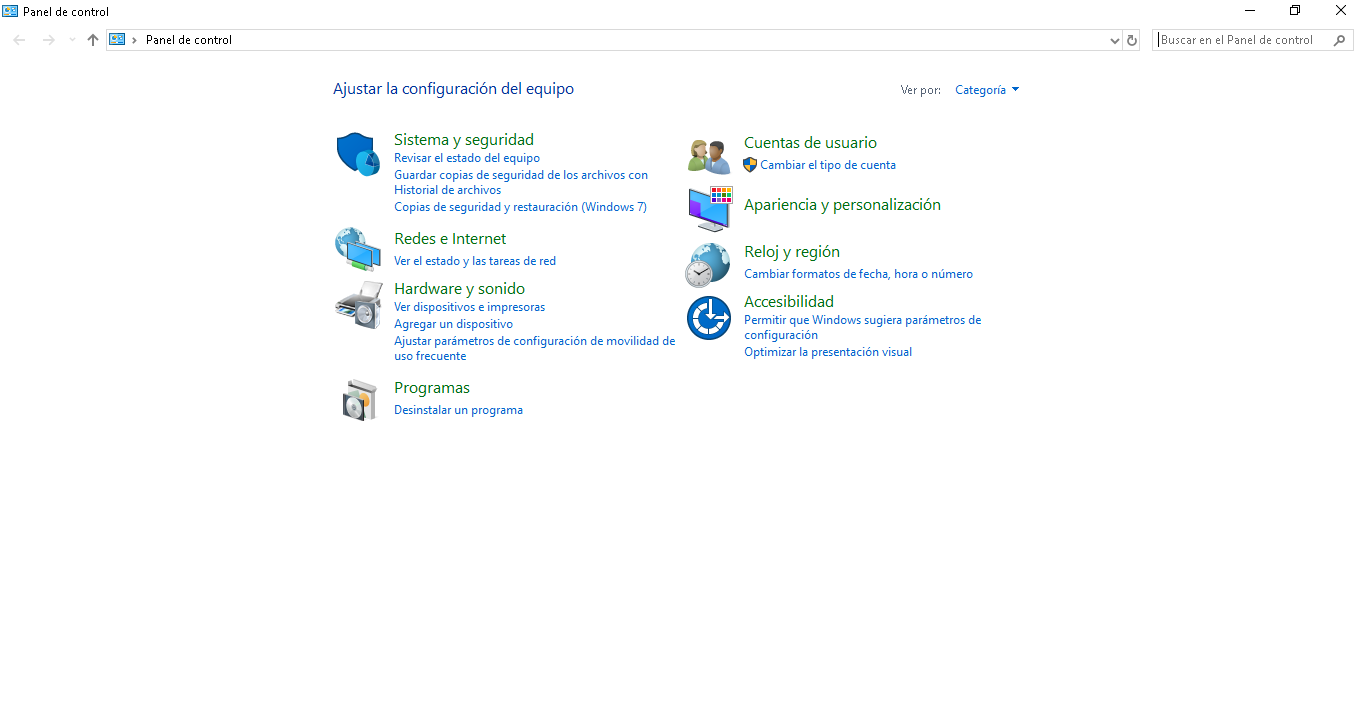
\includegraphics[scale=0.3]{imagenes/cmd/cmd_0.PNG}
    \caption{Abrimos Panel de Control de Windows y entramos a Sistema y Seguridad}
\end{figure}

\begin{figure}[H]
    \centering
    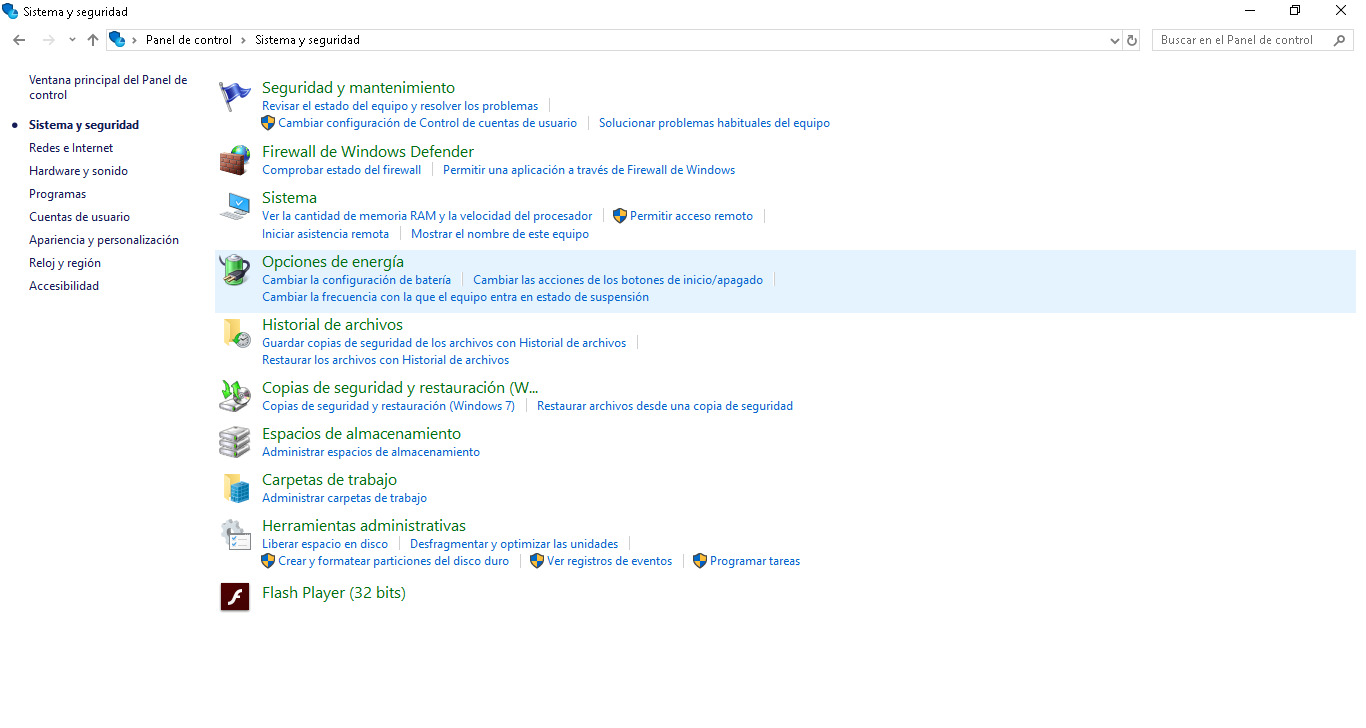
\includegraphics[scale=0.3]{imagenes/cmd/cmd_1.PNG}
    \caption{Entramos en Sistema}
\end{figure}

\begin{figure}[H]
    \centering
    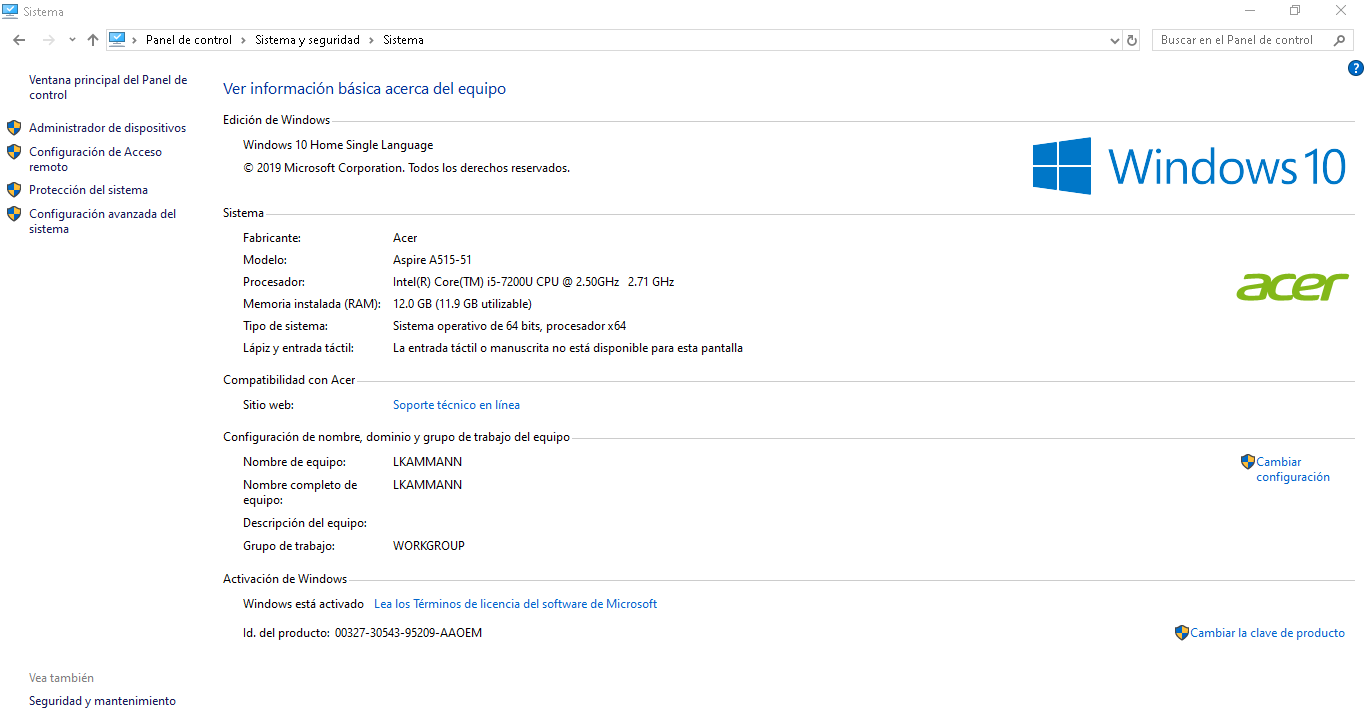
\includegraphics[scale=0.3]{imagenes/cmd/cmd_2.PNG}
    \caption{A la izquierda accedemos en Configuraci\'on avanzada del sistema}
\end{figure}

\begin{figure}[H]
    \centering
    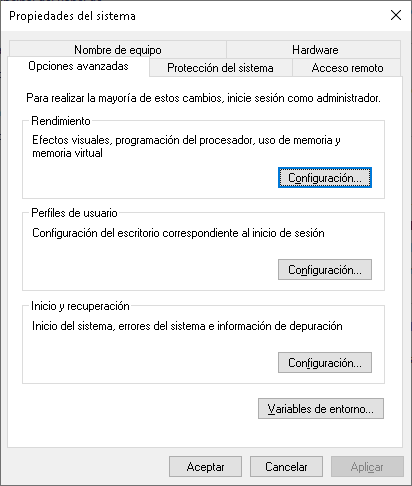
\includegraphics[scale=0.3]{imagenes/cmd/cmd_3.PNG}
    \caption{Entramos en el bot\'on que dice Variables de entorno...}
\end{figure}

\begin{figure}[H]
    \centering
    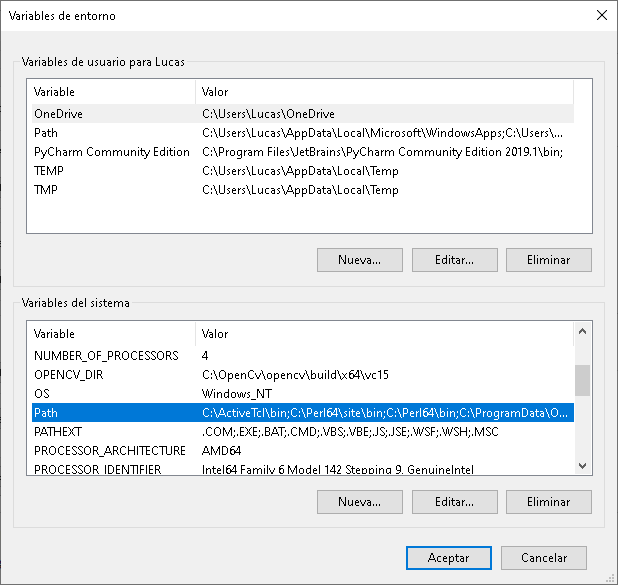
\includegraphics[scale=0.3]{imagenes/cmd/cmd_4.PNG}
    \caption{Buscamos en Variables del sistema la que dice Path}
\end{figure}

\begin{figure}[H]
    \centering
    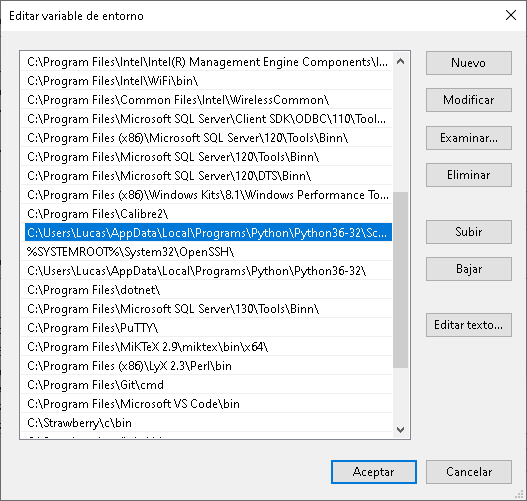
\includegraphics[scale=0.3]{imagenes/cmd/cmd_5.PNG}
    \caption{Accediendo a Path aparecen todo su contenido, tenemos que agregar la ubicaci\'on de Python y sus scripts}
\end{figure}

\begin{figure}[H]
    \centering
    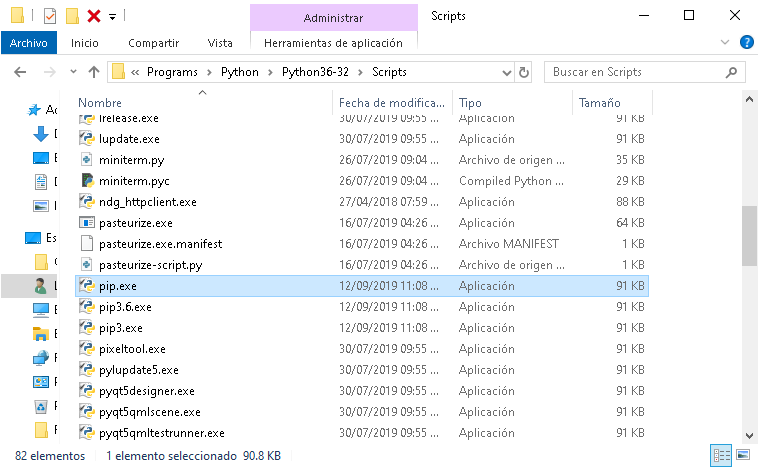
\includegraphics[scale=0.3]{imagenes/cmd/cmd_6.PNG}
    \caption{Ejemplo de la ubicaci\'on de los scripts de Python}
\end{figure}

\subsection{Compilar los dise\~nos de QtDesigner}
\label{compilar_design}
Con la consola de Windows/Linux abierta, posicionado en la carpeta donde tenemos el archivo "*.ui" que creamos y editamos con el QtDesigner,
luego corremos la siguiente l\'inea para compilarlo. Sobre las ventajas o desventajas de este m\'etodo para utilizar los dise\~nos que realizamos en QtDesigner,
es necesario leer otra secci\'on del documento.

\begin{center}
    \textbf{pyuic5 -x filename.ui -o output.py}
\end{center}

\subsection{Compilar los recursos de QtDesigner}
\label{compilar_recurso}
Con la consola de Windows/Linux abierta, posicionado en la carpeta donde tenemos el archivo "*.qrc" que creamos y editamos con el QtDesigner,
luego corremos la siguiente l\'inea para compilarlo.

\begin{center}
    \textbf{pyrcc5 filename.qrc -o output.py}
\end{center}
